\documentclass[12pt,twoside]{article}
\usepackage{jmlda}

\makeatletter
\bibliographystyle{unsrt}
\renewcommand{\@biblabel}[1]{#1.}
\makeatother

%\NOREVIEWERNOTES
\title
    [Аппроксимация фазовой траектории] 
    % Краткое название; не нужно, если полное название влезает в~колонтитул
    {Аппроксимация фазовых траектории квазипериодических сигналов с помощью сферических гармоник}
%\author
 %   [Автор~И.\,О.] % список авторов для колонтитула; не нужен, если основной список влезает в колонтитул
    %{Автор~И.\,О., Соавтор~И.\,О., Фамилия~И.\,О.} % основной список авторов, выводимый в оглавление
    %[Автор~И.\,О.$^1$, Соавтор~И.\,О.$^2$, Фамилия~И.\,О.$^2$] % список авторов, выводимый в заголовок; не нужен, если он не отличается от основного
    %\thanks
    %{Работа выполнена при финансовой поддержке РФФИ, проект \No\,00-00-00000.
   %Научный руководитель:  Стрижов~В.\,В.
   %Задачу поставил:  Эксперт~И.\,О.
   % Консультант:  Консультант~И.\,О.}
%\email
   % {author@site.ru}
%\organization
   % {$^1$Организация; $^2$Организация}
\thanks
	{ }
\abstract
    {\textbf{Аннотация}: Цель данной работы - построить модель аппроксимации наименьшей структурной сложности. Для этогов решается задача аппроксимации фазовой траектории, построенной по квазипериодическому временному ряду.
Фазовая траектория представлена в сферических и декартовых координатах в виде проекции на единичную сферу в пространстве оптимальной размерности.
Оптимальное пространство - это пространство минимальной размерности, в котором фазовая траектория не имеет ярковыроженных самопересечений на поверхности единичной сферы.
Предлагается аппроксимировать полученную фазовую траекторию с помощью сферических гармоник.
Эксперимент проведен на показателях акселерометра мобильного устройства во время ходьбы и бега.  

\bigskip
\textbf{Ключевые слова}: \emph {временные ряды; траекторное подпространство; фазовая траектория; сферические функции}.}

    
\begin{document}
\newcommand{\nsymbol}[2]{\medskip\hangindent=\parindent\hangafter=1\noindent $#1$ --- #2\par}
\newcommand{\nsymbolp}[3]{\nsymbol{#1}{#2 \dotfill\pageref{#3}}}

\newcommand{\hookuparrow}{\mathrel{\rotatebox[origin=t]{270}{$\hookleftarrow$}}}
\newcommand{\hookdownarrow}{\mathrel{\rotatebox[origin=t]{90}{$\hookleftarrow$}}}

\maketitle

\section{Введение}
Ставится задача построения модели аппроксимации квазипериодического временного ряда. Примерами таких сигналов являются показания акселерометра во время ходьбы и бега.
	
Для этого строится пространство фазовой тракеториии по выбранному временному ряду.  Это делается с помощью построения траекторной матрицы или матрицы Ганкеля.
Для нашего исследования 
Размерность траекторного пространства может оказаться избыточна. Это может приводить к неустойчивости исследуемых моделей и сложному описанию временного ряда. Для понижения размерности фазового пространства предлагается для сравнения использовать  различные линейные и нелинейные методы рассмотренные в \cite{Maaten2007}.
	
В выбранном пространстве уменьшенной размерности предлагается спроецировать имеющуюся траекторию на $p$-мерную единичную сферу и перейти в $p-1$-мерное сферическое пространство. Полученную определенную на поверхности сферы функцию предлагается представить в виде ряда разложенного по сферическим функциям.

\begin{figure}[h]
\centering
  \subfloat[Временной ряд]{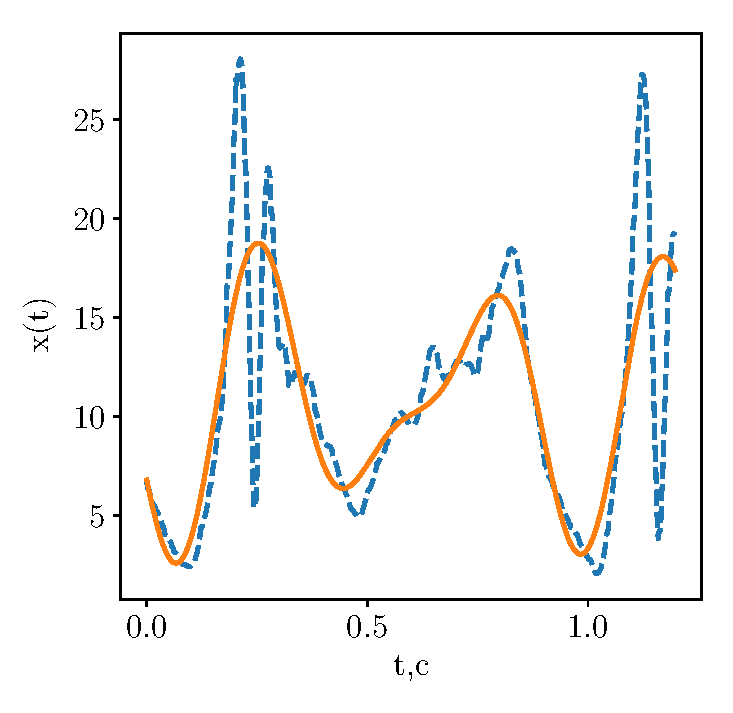
\includegraphics[width=0.3\textwidth]{figs/tr_init}}
  \subfloat[Фазовая траеткория (PCA)]{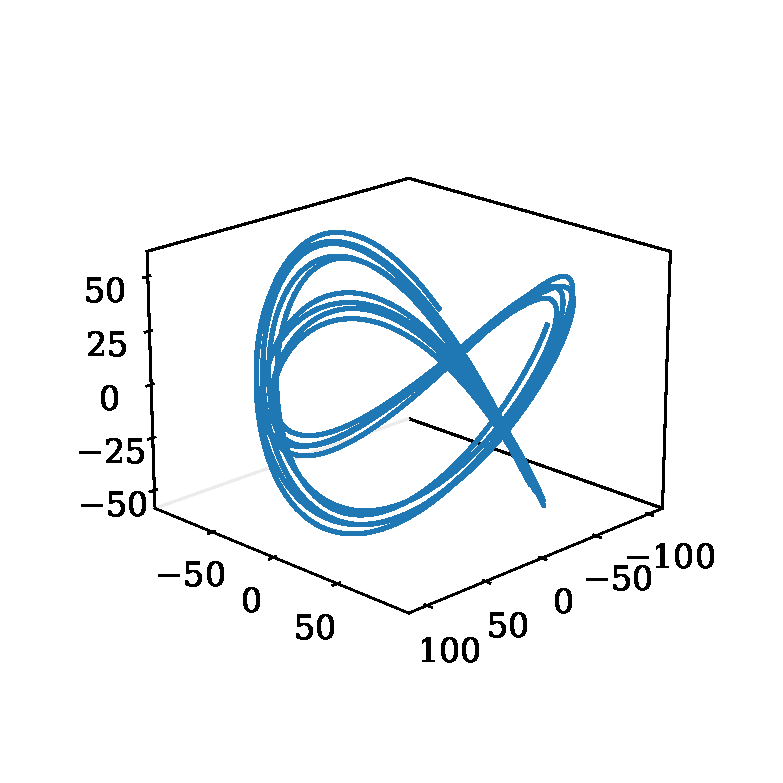
\includegraphics[width=0.3\textwidth]{figs/phase_init}}\\
\caption{Исследуемый временной ряд и его фазовая траетория. }
\label{fg:initial_traj}
\end{figure}

На рис.~\ref{fg:initial_traj} показан изначальный временной ряд и его разложение, пунктирной и сплошной линией соответственно, а также его фазовая траектория уменьшенная в пространство размерности 3 с помощью метода главных компонент (principal component analysis, PCA).

\section{Постановка задачи}
По имеющемуся временному ряду $\mathbf{s}=[s_1,...,s_N]^{\mathsf{T}}$ строится траекторная матрица или матрица Ганкеля

\begin{equation}
\mathbf{H_{s}} = 
\begin{bmatrix} 
	s_{1} & s_{2} & \ldots &s_{n-1} &s_{n}\\
	s_{2} & s_{3} & \ldots &s_{n} &s_{n+1}\\
	\vdots& \vdots & \ddots & \vdots & \vdots\\
	s_{N-n+1} & s_{N-n+2} &\ldots&s_{N-1} &s_{N}\\
\end{bmatrix}
\label{eq:hankel_matrix}
\end{equation}
                   
где $N$-длинна временного ряда, $n$-ширина окна, не меньшая, чем предполагаемый период. Обозначим $t$-ую строку матрицы Ганкеля $\mathbf{H_{s}}$ за $\mathbf{x_{t}}$. Матрица $\mathbf{H_{s}}$ пребразуется к:	
\begin{equation}
	\mathbf{H_{s}} = 
	\begin{bmatrix} 
                  	\mathbf{x_{1}}\\ \mathbf{x_{2}}\\
                  	\vdots\\
                  	\mathbf{x_{m}}\\
                   \end{bmatrix},
                   \mathbf{x_t}=[s_{t},s_{t+1},\ldots,s_{t+n-1}] ,
                   m = N-n+1
\label{eq:hankel_matrix_2}
\end{equation}
\vspace{\baselineskip}

Все векторы $\mathbf{x_{t}}$ принадлежат $\mathbb{H}_{\mathbf{x}} \subseteq \mathbb{R}^{n}$. Предполагается, что размерность траекторного пространства избыточна, поэтому предлагается исследовать некоторые проекции на траекторное подпространство.
Однако заранее неизвестно, в каком пространстве необходимо уменьшать размерность, поэтому задача приобретает следующий состоящий из двух вариантов вид:

\begin{equation}
	t \mapsto \mathbf{x} \mapsto \mathbb{H}_{x}^{n} \xrightarrow{} \mathbb{H}_{x}^{p} \xrightarrow{} \mathbb{S}_z^{(p-1)} \hookrightarrow [0,2\pi] \xrightarrow{f} r
\label{eq:goal}
\end{equation}

\begin{equation}
	t \mapsto \mathbf{x} \mapsto \mathbb{H}_{x}^{n} \xrightarrow{} \mathbb{S}_z^n \xrightarrow{} \mathbb{S}_z^{(p-1)} \hookrightarrow [0,2\pi] \xrightarrow{f} r
\label{eq:goal_2}
\end{equation}

При понижении пространства, во-первых, требуется отыскать подходящий способ снижения размерности (линейные, нелинейные, нейросетевые методы), во-вторых, необходимо определить в каком пространсве сокращение размерности приведет к наименьшей потери информации и далее найти оптимальной сложности приближение при отысканию вложений. 
\vspace{\baselineskip}

\begin{Def}
Параметрическая аппроксимирующая модель временного ряда  $\mathbf{x}$  - это такое отображение $g$, что:
\begin{equation}
	g: \mathbb{R}^{q} \times \mathbf{S} \xrightarrow{} \mathbf{S}
\label{eq:param_model}
\end{equation}
\end{Def}

Предполагается, что аппроксимирующая модель строится в пространстве меньшей размерности $(p-1)$, в котором выбранное отображение $h: \mathbf{H}_{x}^{n} \xrightarrow{} \mathbf{S}_x^{(p-1)} $, где $(p-1)\ll n$, сохраняет геометрическую структуру множество точек $\mathbf{H}_{x}^{n}$. 

\begin{Def}
Структурная сложность - это количество параметров $q$ модели, позволяющих строить адекватную аппроксимацию.
\end{Def}



\section{Понижение размерности}
\paragraph{Алгоритмы понижения размерности}
Рассматриваемый поход предполагает использование и анализ различных алгоритмов понижения размерности согласно \cite{Maaten2007}.
Предполагается, что исследуемые способы относятся к различным семействам алгоритмов понижения размерности и позволяют качественно отыскивать одномерные многообразия в многомерных пространствах.

Используется алгоритм Kernel Principal Component Analysis (KPCA), описанный в \cite{Scholkopf1998, Ezukwoke2019}, позволяющий обобщить классический PCA с помощью нелинейных преобразиваний $\Phi$ матрицы несмещенных данных $\mathbf{x}_i, ~i=1,...,m,~\mathbf{x}_i \in \mathbb{R}^n$:

\begin{equation}
	 C = \frac{1}{m}\sum_{i=1}^{m}\Phi(\mathbf{x}_i) \Phi(\mathbf{x}_i)^T,
	 \qquad \sum_{i=1}^{m}\Phi(\mathbf{x}_i) = 0,
	 \qquad \Phi: \mathbb{R}^{n} \xrightarrow{} \mathbb{R}^{n'},
	 \quad n\ll n'
\label{eq:kpca}
\end{equation}

Далее применяется ядерный метод позволяющий избегать явного отображения в новое пространство высокой размерности, включающий в себя матрицу Грама $\mathbf{K} \in \mathbb{R}^{m \times m}$ и функцию ядро $k$. Для нахождения итогового отображения в пространство малой размерности находятся собственные значения и собственные вектора матрицы $\mathbf{\tilde K}$, если данные не центрированы. 

\begin{equation}
	 \mathbf{K}_{i,j} = k(\mathbf{x}_i,\mathbf{x}_j) = \Phi(\mathbf{x}_i)^T\Phi(\mathbf{x}_j),
	 \quad \mathbf{\tilde K} = \mathbf{K} - \mathbf{1}_m\mathbf{K} - \mathbf{K} \mathbf{1}_m  +\mathbf{1}_m\mathbf{K}\mathbf{1}_m,
\label{eq:K_matrix}
\end{equation}
где  $\mathbf{1}_m$ - это матрица $m\times m$, в которой каждый элемент равен $1/m$.

Применяются следующие базовые варианты ядерной функции $k$.

\begin{itemize}
\item \textbf{Линейное ядро (англ. linear)}
\begin{equation}
	k(\mathbf{x}_i,\mathbf{x}_j) = \mathbf{x}_i\mathbf{x}_j^T,
\label{eq:kernel_linear}
\end{equation}
это ядро приводящее KPCA к классическому линейному PCA.
\end{itemize}

\begin{itemize}
\item \textbf{Полиномиальное ядро (англ. polynomial или poly)}
\begin{equation}
	k(\mathbf{x}_i,\mathbf{x}_j) = (\mathbf{x}_i\mathbf{x}_j^T + c)^d,
	\quad d \ge 0,
	\quad c \ge 0
\label{eq:kernel_poly}
\end{equation}
%где $c > 0$, \; $c = const$, \; $d \ge 1$ - степень полинома.
\end{itemize}

\begin{itemize}
\item \textbf{Гауссово ядро (англ. Radial basis function, rbf)}
\begin{equation}
	k(\mathbf{x}_i,\mathbf{x}_j) = exp\left(-\frac{||\mathbf{x}_i-\mathbf{x}_j||^2}{2\sigma^2}\right),
	\quad \sigma > 0
\label{eq:kernel_rbf}
\end{equation}
%где  $\sigma > 0$.
\end{itemize}

\begin{itemize}
\item \textbf{Cигмоидальное ядро (англ. sigmoid)}
\begin{equation}
	k(\mathbf{x}_i,\mathbf{x}_j) = tanh(\gamma(\mathbf{x}_i\mathbf{x}_j^T) + c),
	\quad \gamma > 0,
	\quad c\ge0
\label{eq:kernel_sigmoid}
\end{equation}
%где  $\gamma > 0$, \; $c\ge0$.
\end{itemize}

\begin{itemize}
\item \textbf{Косинусное ядро (англ. cosine)}
\begin{equation}
	k(\mathbf{x}_i,\mathbf{x}_j) = \frac{\mathbf{x}_i\mathbf{x}_j^T}{||\mathbf{x}_i||~||\mathbf{x}_j||}
\label{eq:kernel_cosine}
\end{equation}
\end{itemize}

\paragraph{Фазовые траектории в пространстве малой размерности}

\begin{figure}[h]
\centering
  \subfloat[KPCA cosine]{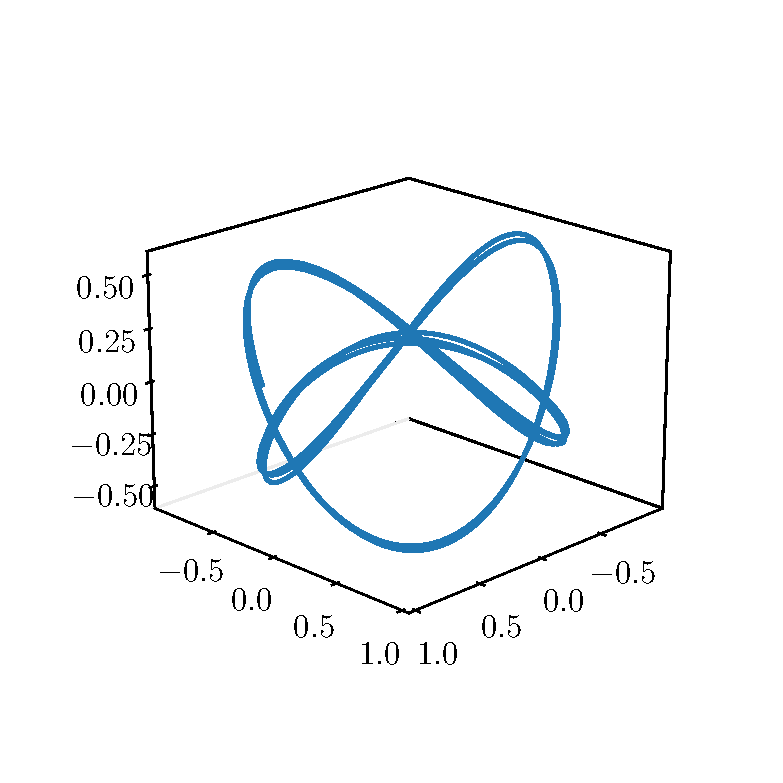
\includegraphics[width=0.25\textwidth]{figs/phase_cosine}}
  \subfloat[KPCA poly]{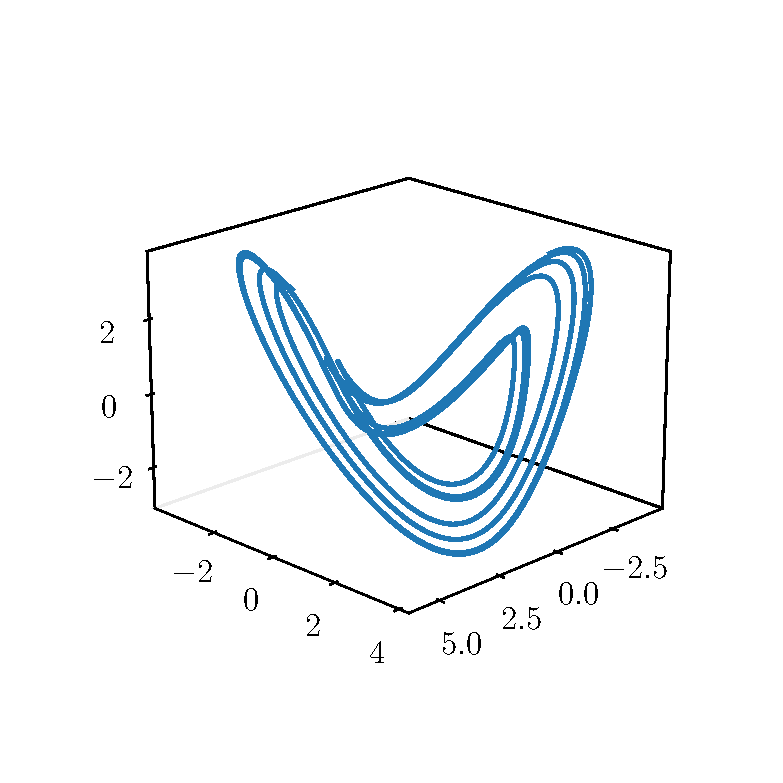
\includegraphics[width=0.25\textwidth]{figs/phase_poly}}
  \subfloat[KPCA rbf]{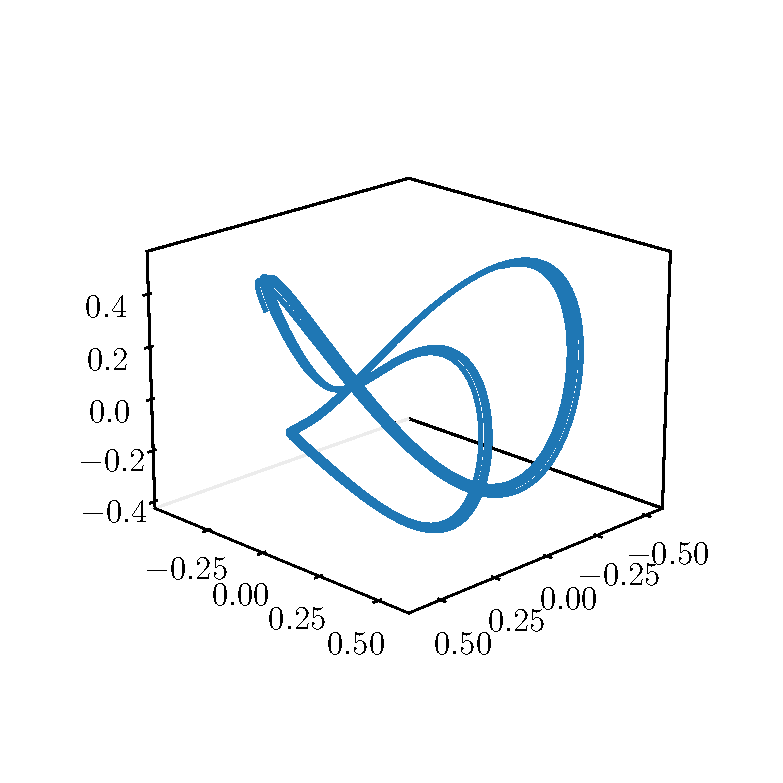
\includegraphics[width=0.25\textwidth]{figs/phase_rbf}}
  \subfloat[KPCA sigmoid]{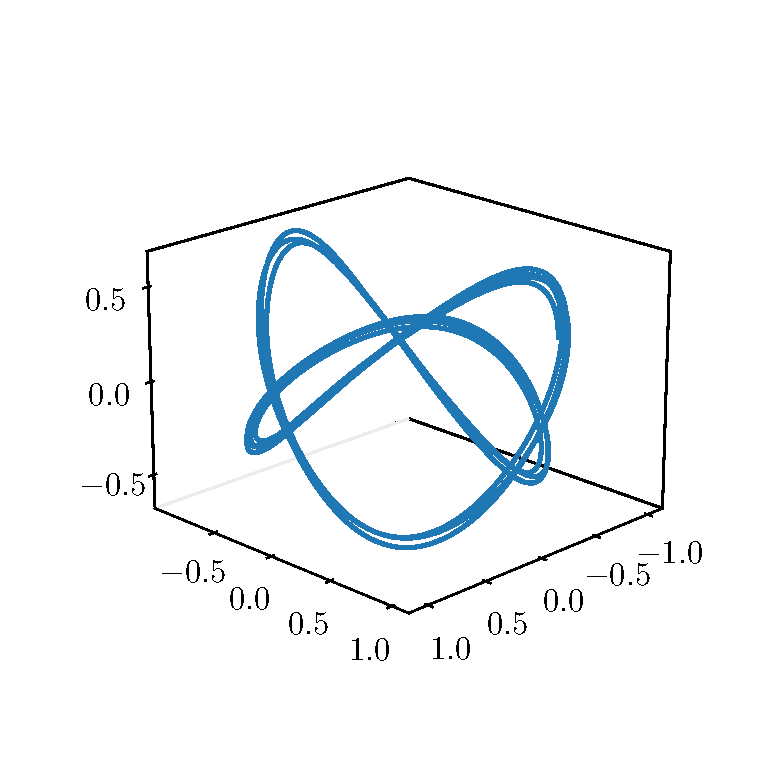
\includegraphics[width=0.25\textwidth]{figs/phase_sigmoid}}\\
  \subfloat[t-SNE]{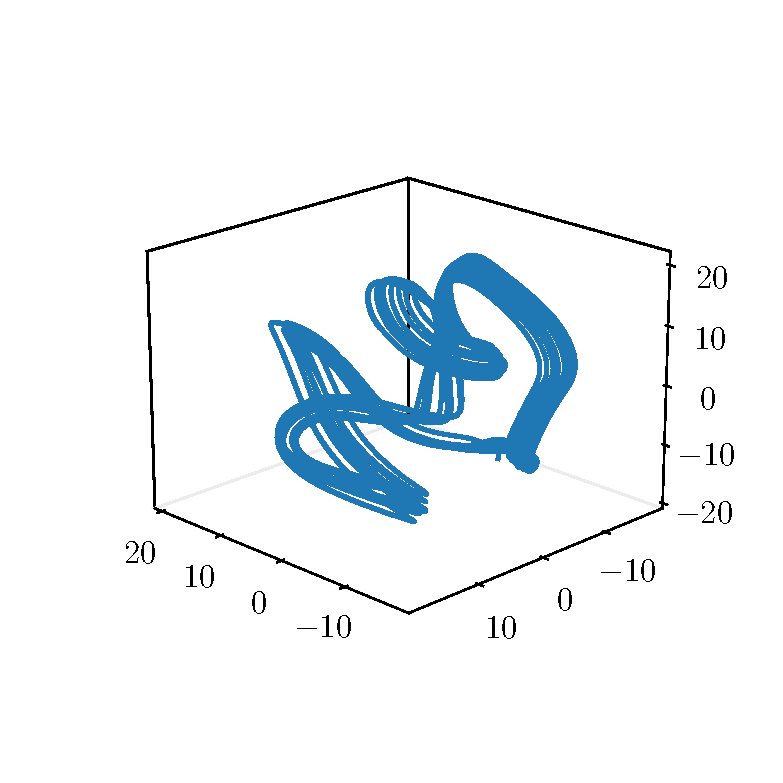
\includegraphics[width=0.25\textwidth]{figs/phase_tsne}}
  \subfloat[Autoencoder]{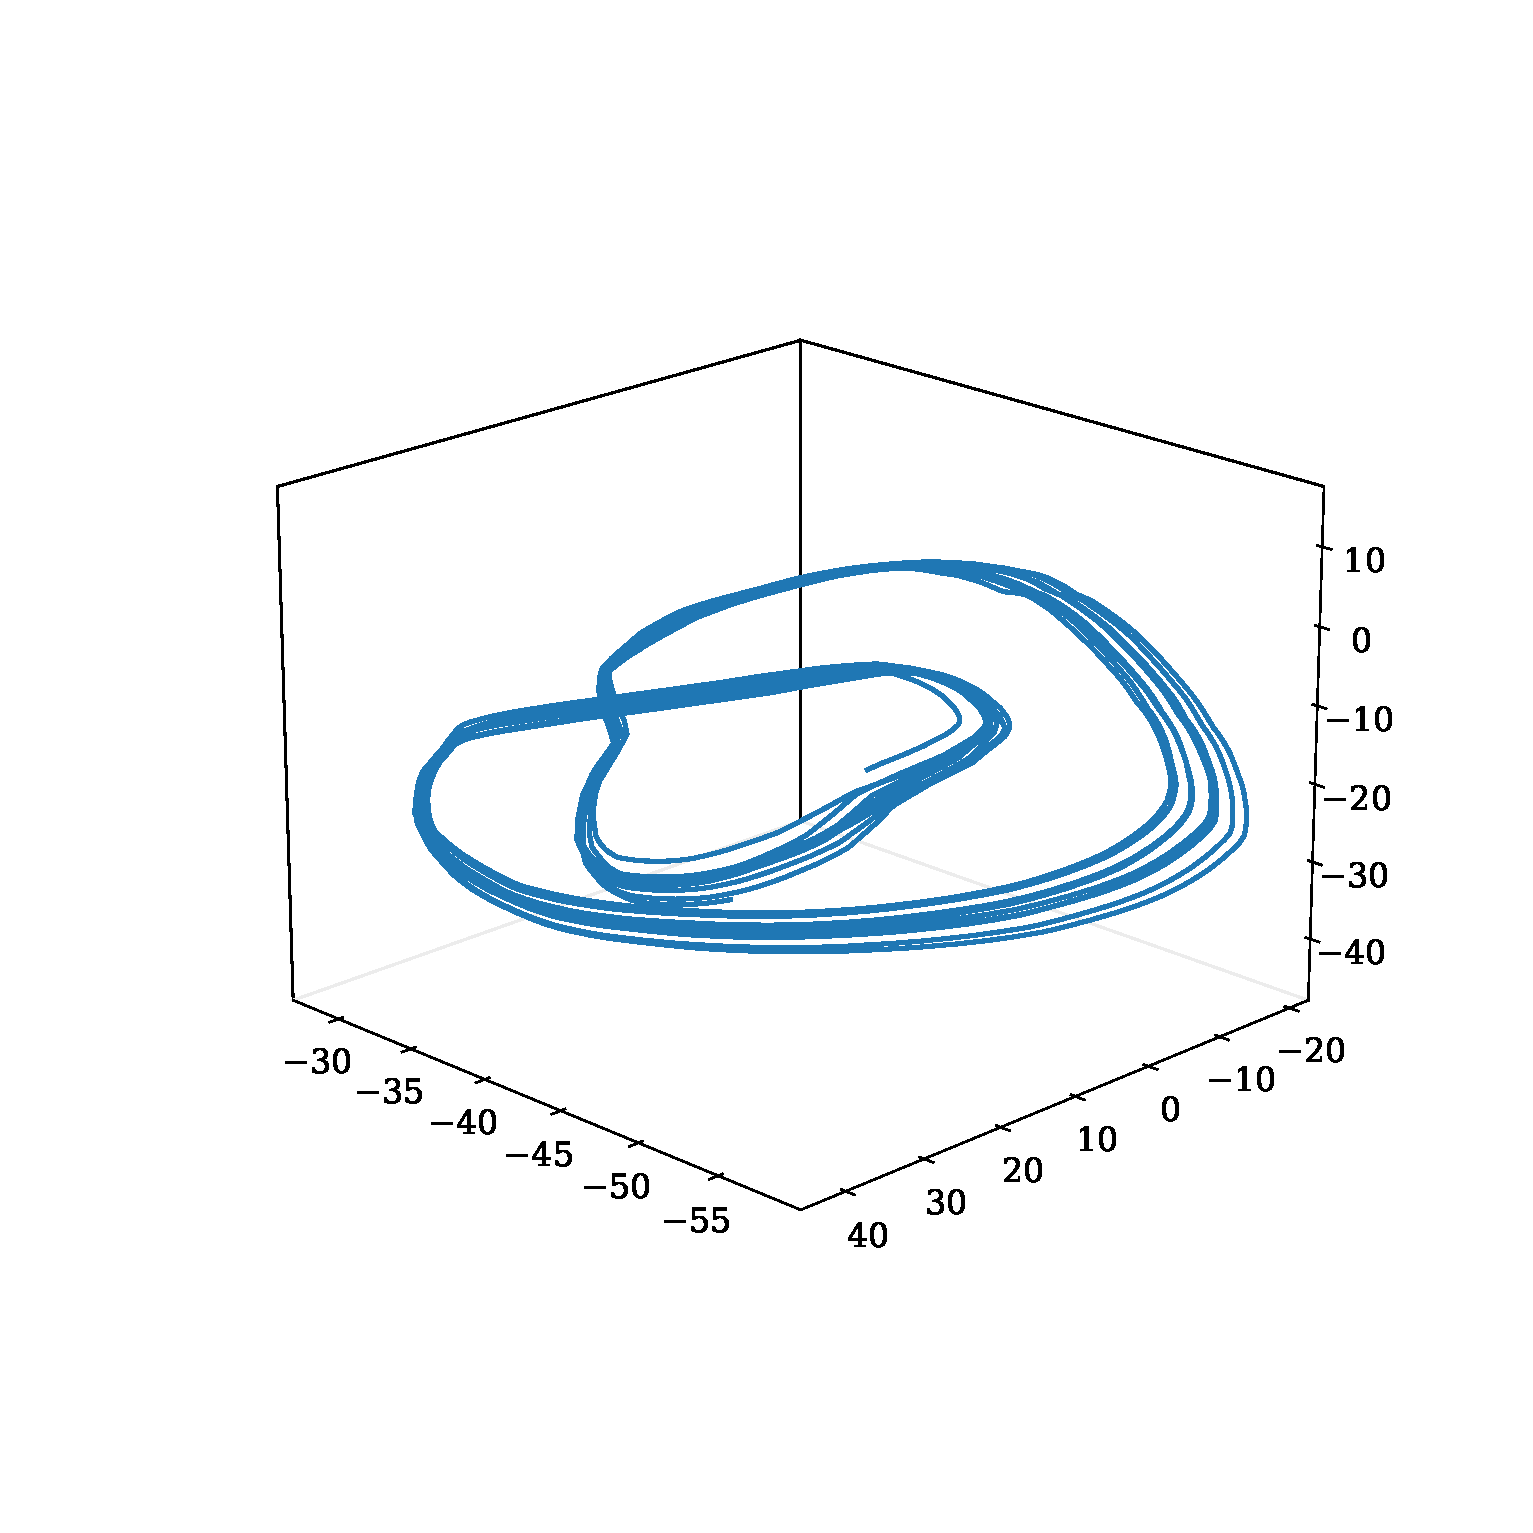
\includegraphics[width=0.25\textwidth]{figs/phase_enc}}
  \subfloat[MDS]{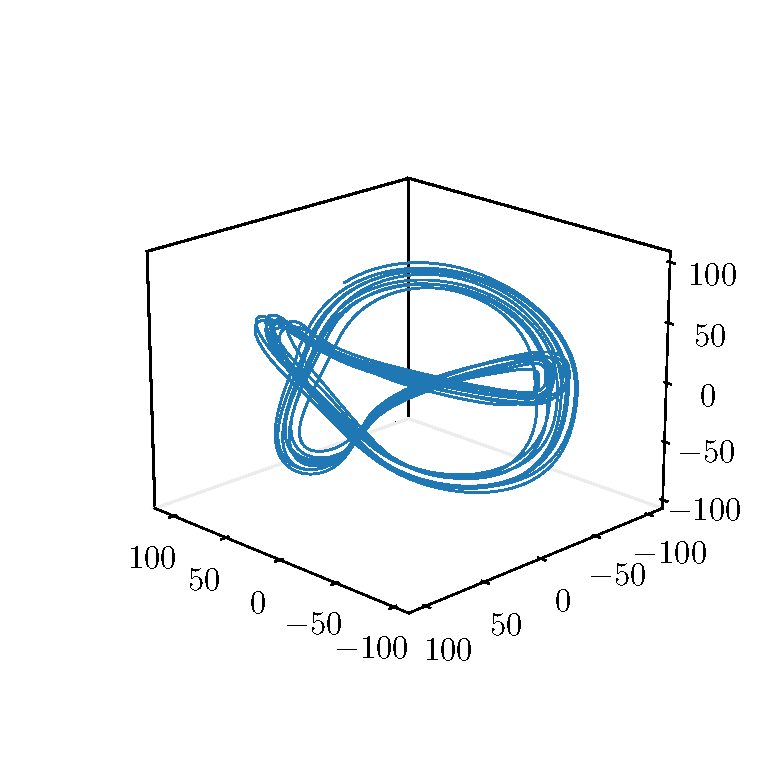
\includegraphics[width=0.25\textwidth]{figs/phase_mds}}
  \subfloat[Hessian LLE]{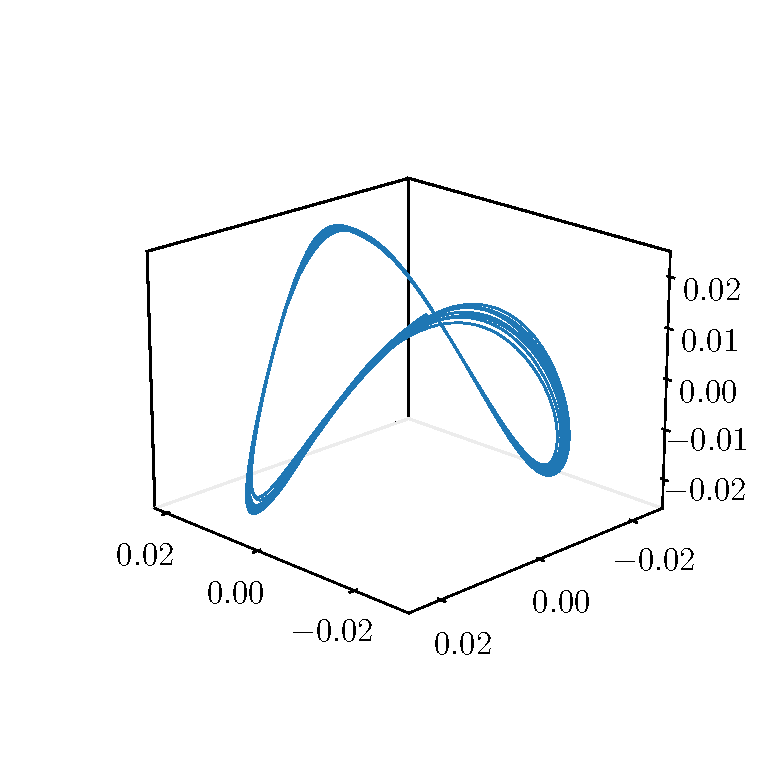
\includegraphics[width=0.25\textwidth]{figs/phase_hLLE}}
\caption{Уменьшениt размерности фазовой траектории в декартовых координатах. }
\label{fg:new_traj_1}
\end{figure}

Некоторые из исследуемых моделей уже можно использовать в качестве аппроксимационных, так как с помощью координат в уменьшенном пространстве можно задавать вид фазовой траектории для различных типов движения.

\vspace{\baselineskip}
\begin{table}
    \caption{MAPE восстановленной траектории.}
    \label{accuracy_table}
    \centering\medskip%\tabcolsep=2pt%\small
    \begin{tabular}{lrrrrrrrr}
    \headline
        Алгоритм
            & \multicolumn{1}{c}{p=2}
            & \multicolumn{1}{c}{p=3}
            & \multicolumn{1}{c}{p=4}
            & \multicolumn{1}{c}{p=5}
            & \multicolumn{1}{c}{p=6}
            & \multicolumn{1}{c}{p=7} \\
    \headline
        {\tt PCA}
        %
            & $-$ & $-$ & $-$ & $-$ & $-$ & $-$  \\
        {\tt KPCA Cosine}
        %['cosine', 46.354525124885235, 38.5077616060247, 29.618070613903885, 28.841379209863078, 28.49246588499732, 28.544181696163562]
            & $46.35$ & $38.50$ & $29.61$ & $28.84$ & $28.49$ & $28.54$  \\
        {\tt KPCA poly}
        %['poly', 46.36673685589005, 36.86006190524614, 22.227530065869043, 20.02710668177695, 19.25438646356014, 17.94444510766801]
            & $46.36$ & $36.86$ & $22.22$ & $20.02$ & $19.25$ & $17.94$  \\
        {\tt KPCA rbf}
        %['rbf', 45.55393369086398, 45.36468017153293, 44.93575581137207, 44.823243893388344, 44.503472447925944, 44.56293823719358]
            & $45.55$ & $45.36$ & $44.93$ & $44.82$ & $44.50$ & $44.56$  \\
        {\tt KPCA sigmoid}
        %['sigmoid', 47.04786679981016, 47.04786679981016, 47.04786679981016, 47.04786679981016, 47.04786679981016, 47.04786679981016]
            & $47.04$ & $47.04$ & $47.04$ & $47.04$ & $47.04$ & $47.04$  \\ 
	{\tt  t-SNE}
	%
            & $-$ & $-$ & $-$ & $-$ & $-$ & $-$  \\      
         {\tt  Autoencoder}
         %
            & $-$ & $-$ & $-$ & $-$ & $-$ & $-$  \\  
         {\tt  MDS}
         %
            & $-$ & $-$ & $-$ & $-$ & $-$ & $-$  \\  
         {\tt  Hessian LLE}
         %
            & $-$ & $-$ & $-$ & $-$ & $-$ & $-$  \\       
                                             
    \hline
    \end{tabular}
\end{table} 
В таблице~\ref{accuracy_table} сравним точности различных алгоритмов в смысле точности восстановления изначальной траектории согласно MAPE:
\begin{equation}
\textrm{MAPE}\mathbf{({x,\hat{x}})} =  \frac{100\%}{n}\sum_{t=1}^{n}\left |\frac{x_t - \hat{x}_t}{x_t}\right|
\label{eq:mape}
\end{equation}
\section{Модели аппроксимации}
\paragraph{GAN для фазовых траекторий в 2D}

\begin{itemize}
\item \textbf{Модель генератор реальных данных}
\begin{equation}
	t \xrightarrow{} s\xrightarrow{Hankel}  \mathbf{x}_i \xrightarrow{PCA} x_i,
	\label{eq:GAN_real}
\end{equation}
где $x_i$ - точка фазовой траектории в уменьшенном пространстве, $x_i \in \mathbb{R}^2$.
\end{itemize}

\begin{itemize}
\item \textbf{Модель генератор синтетических данных}

\begin{equation}
	f_{ph}(\mathbf{w},\phi) = \sum_{j=0}^{l} w_{0,j}cos(j\phi) + i w_{1,j}sin(j\phi),
\label{eq:f_ph}
\end{equation}

\begin{equation}
	\phi \xrightarrow{f_{ph}} \hat{x}_{\phi},
	\quad
	\hat{x}_{\phi} = [real(f_{ph}),\:imag(f_{ph})],
	\quad
	\hat{x}_{\phi}  \in \mathbb{R}^2,
\label{eq:GAN_fake_1}
\end{equation}
\vspace{\baselineskip}

где $\mathbf{w}$ - вектор параметров (коэффициентов) тригонометрического ряда, $l$-количество пар коэффициентов.

Восстановление изначального временного ряда с помощью $f_{ph}$ можно представить в виде
\begin{equation}
	\phi \xrightarrow{f_{ph}} \hat{x}_{\phi} \xrightarrow{inverse~PCA}  \mathbf{x}_i \xrightarrow{inverse~Hankel}s
\label{eq:GAN_fake_2}
\end{equation}
\end{itemize}

\begin{itemize}
\item \textbf{Дискриминатор или функция потери и оптимизация}

Функцию потерь представляется в виде
\begin{equation}
\textrm{Loss}\mathbf{(\hat{x}_{\phi},x)} =  \sum_{i=1}^{101}\sum_{j=1}^{k}(\hat{x}_{\phi,i} - x_{i,j})^2
\label{eq:L}
\end{equation}
где для любого фиксированного $i$\; $\{x_{i,j}\}_1^k$ -- $k$ ближайших соседей к $\hat{x}_{\phi,i}$.

Решается задача оптимизации:
\begin{equation}
\mathbf{\hat{w}} = \argmin_{\mathbf{w} \in \mathbb{R}^{2l}} \textrm{Loss}(\mathbf{w}|\{x\})
\label{eq:arg_l}
\end{equation}
\end{itemize}

\paragraph{GAN для фазовых траекторий в 3D}

Предполагается, что структура модели проще в сферических координатах.
Построим отображение $x_p \in \mathbb{H}_{x}^{p} $ в $\mathbb{S}_{z}^{p-1} $ при $p = 2$.

\begin{equation}
	\phi: \mathbf{x}_p(t)  \xrightarrow{} \mathbf{z}_{(p-1)}(t) = [\alpha_{1} (t),..., \alpha_{p-1}(t), r{t}]
\label{eq:param_model2}
\end{equation}

В качестве базисных функций на поверхности 3 мерной сферы выберем сферические гармоники:

\begin{equation}
	Y_l^m(\alpha_1,\alpha_2) = \sqrt{ \frac{(2l+1)}{4\pi} \frac{(l-m)!}{(l+m)!} } P_l^m(cos\theta)e^{im\phi}
\label{eq:Yml}
\end{equation}

\begin{itemize}
\item \textbf{Модель генератор синтетических данных}

\begin{equation}
	f_{ph}(\mathbf{w},\alpha_1,\alpha_2) = \sum_{n,m \in N,M} w_{n,m}Y_l^m(\alpha_1,\alpha_2)
\label{eq:f_ph_3d}
\end{equation}
\vspace{\baselineskip}

\item \textbf{Дискриминатор или функция потери и оптимизация}

Функцию потерь представляется в виде
\begin{equation}
\textrm{Loss} =  \sum_{n,m \in N,M} \hat{f}_{ph}(\mathbf{w},\alpha_1,\alpha_2) - f_{real}(\alpha_{1},\alpha_2)
\label{eq:L_3d}
\end{equation}

Решается задача оптимизации:
\begin{equation}
\mathbf{\hat{w}} = \argmin_{\mathbf{w} \in \mathbb{R}^{2l}} \textrm{Loss}(\mathbf{w}|\{z_{2}\})
\label{eq:arg_l}
\end{equation}
\end{itemize}


\section{Эксперимент}

\paragraph{Аппроксимация сферическими гармониками 3D}

\begin{figure}[h]
\centering
\includegraphics[width=0.5\textwidth]{figs/3D_sp_harm}
\caption{Аппроксимация сферическими гармониками 3D. }
\label{fg:3D_sp_harm}
\end{figure}

\section{Заключение}
\newpage
\bibliographystyle{unsrt}
\bibliography{lib}

\end{document}
